\section{Dynamic Bayesian Networks}
\subsection{Definition}
\begin{frame}
%\frametitle{Dynamic Bayesian Networks}
\begin{definition}
        A DBN is a pair $(B_0, B_{\rightarrow})$, where $B_0$ is a Bayesian network over $\chi^{(0)}$ representing the initial distribution, and $B_{\rightarrow}$ is a 2-TBN for the process. For any desired time span $T \geq 0$, the distribution over $\chi^{(0:T)}$ is defined as a unrolled Bayesian network, where, for any $i=1,...,n$:
        \begin{itemize}
        \item the structure and CPDs of $X_i^{(0)}$ are the same as those for $X_i$ in $B_0$,
        \item the structure and CPDs of $X_i^{(t)}$ for $ t \geq 0 $ are the same as those for $X_i^{'}$ in $B_\rightarrow$.
        \end{itemize}
\end{definition}
\end{frame}

\subsection{Example}
\begin{frame}
%\frametitle{Example}
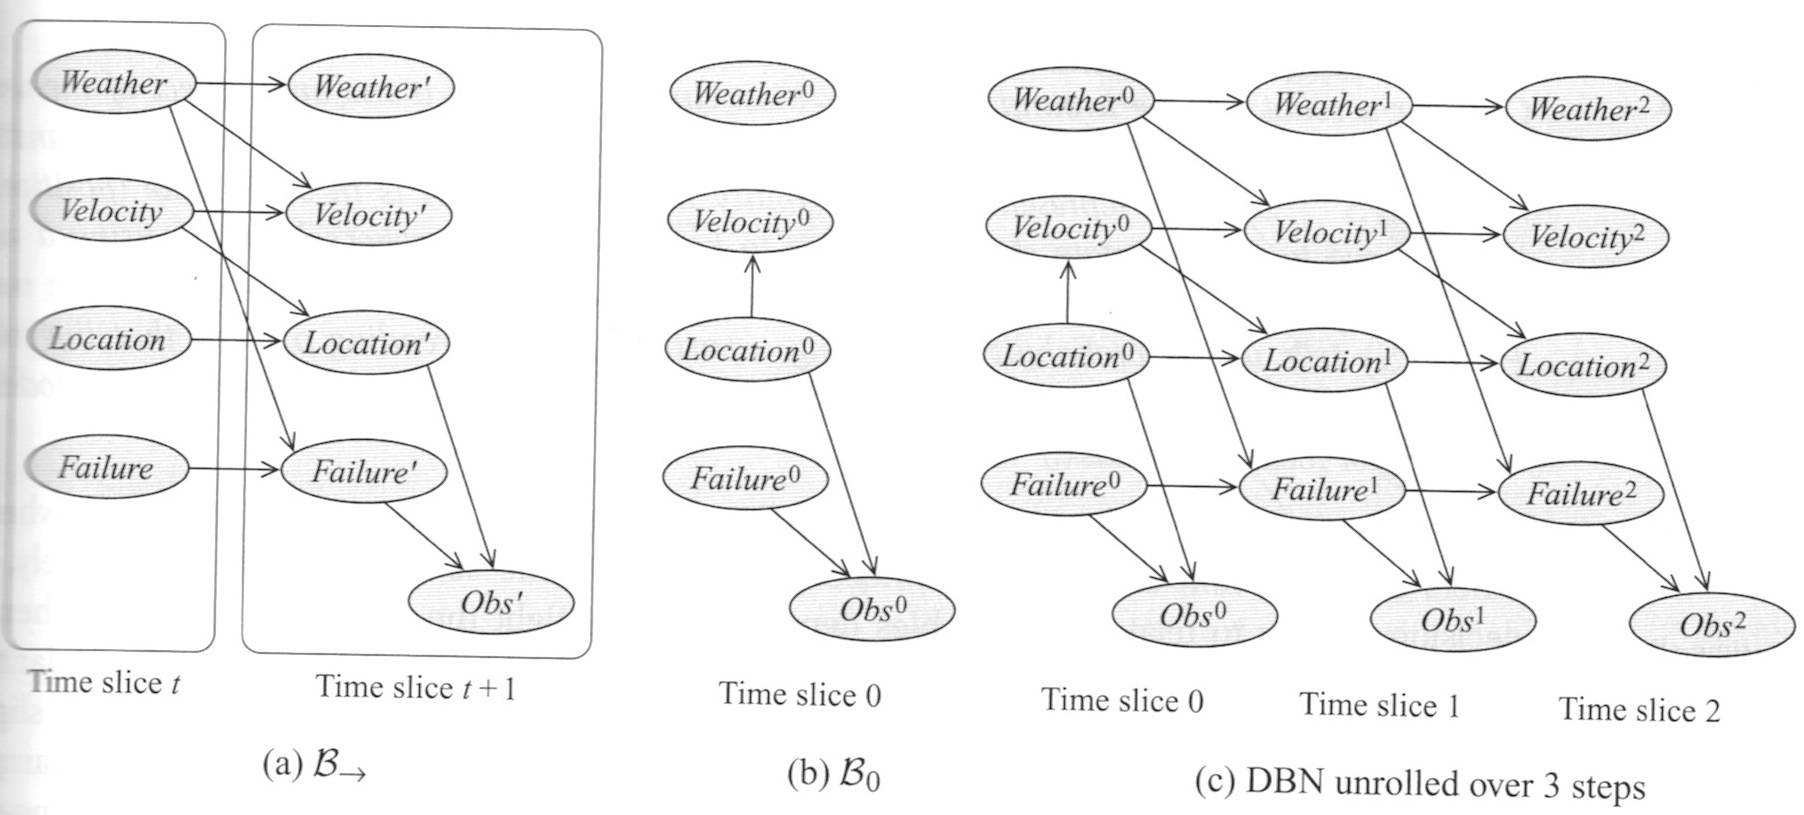
\includegraphics[width=.9\textwidth]{figures/dbn}
\end{frame}

\subsection{Inference}

\begin{frame}
\frametitle{Exact Inference}
\begin{itemize}
\item We can use standard inference algorithms (e.g. variable elimination)
\item Problem I: run inference on larger an larger networks over time
\item Problem II: maintain our entire history of observations indefinitely
\item Solution/workaround: use approximate inference
\end{itemize}
\end{frame}

\begin{frame}
\frametitle{Approximate Inference}
\begin{itemize}
\item We can use some kind of Likelihood Weighting
\item Two modifications:
\begin{enumerate}
\item run all samples together through the DBN, one slice at a time
\item focus the set of samples on the high-probability regions of the state space
\end{enumerate}
\item Particle Filter:
\begin{enumerate}
\item Each sample is propagated forward by sampling the next state value $x_{t+1}$ given the current value $x_t$ for the sample
\item Each sample is weighted by the likelihood it assigns to the new evidence $P(e_{t+1}|x_{t+1})$
\item The population is \textit{resampled} to generate a new population of $N$ samples. Each new sample is selected from the current population; the probability that a particular sample is selected is proportional to its weight.
\end{enumerate}
\end{itemize}
\end{frame}

\begin{frame}
\frametitle{Algorithm}
\end{frame}